\chapter{Results and Discussion}

\section{Sequences and Static Structures}
\begin{figure}[h!]
	\label{MSA matrix}
	\centering
	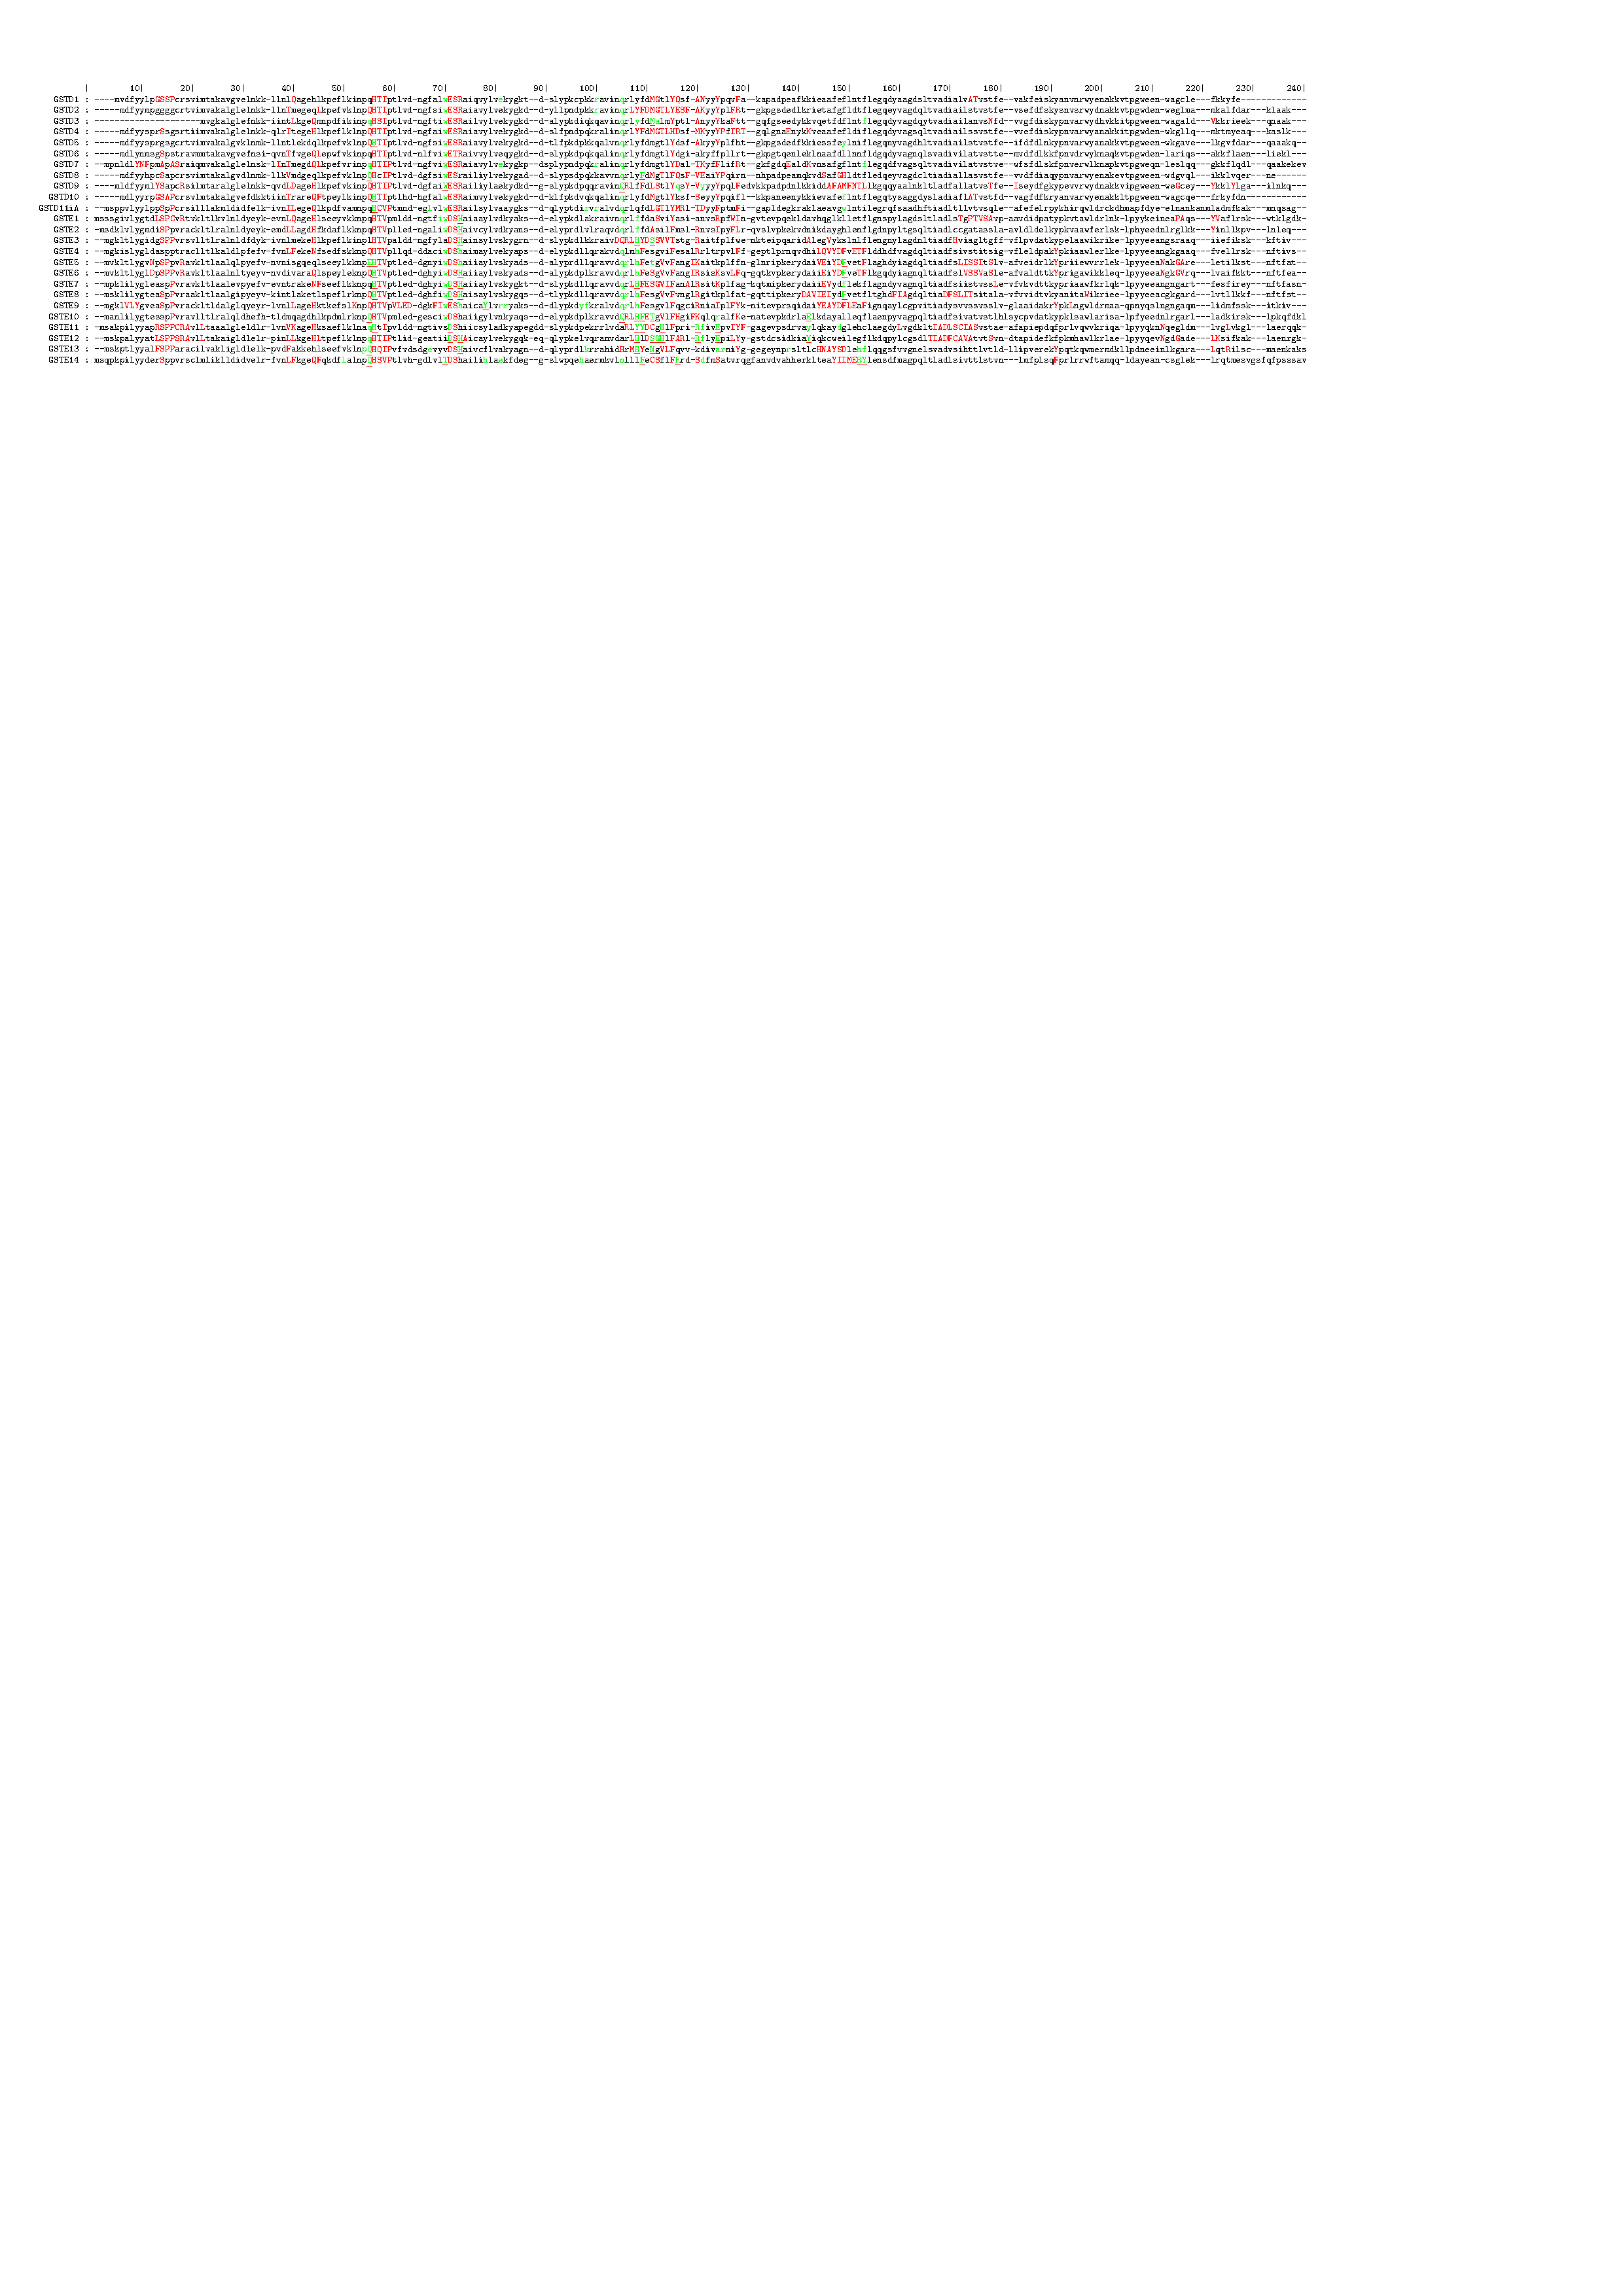
\includegraphics[width = 0.99\linewidth]{figures/fig1}
	\caption{MSA, each line of this matrix corresponds to a given sequence of interest and each column gives the aligned residue that is associated to this sequence. Amino-acids that have been identified as part of the interface of dimerization in the AlphaFold structures are displayed in red upper case. Amino-cadis that have been identified as part of the binding site in the AlphaFill structure are displayed in green.}
\end{figure}
The figure (\ref{MSA matrix}) represents the computed sequence alignment obtained with the $25$ GSTs.
\section{Dynamics from Normal Modes}

\section{Dynamic from Molecular Dynamics}

\section{Comparison between Structures}